\documentclass[aspectratio=169, 14pt]{beamer}
\usetheme{TalentSprint}
\usepackage{tcolorbox}
\usepackage{booktabs}
\usepackage{amsmath}
\usepackage{tikz}
\usetikzlibrary{shapes, shadows, arrows}
\tikzstyle{arrow} = [thick, ->, >=stealth, color =black,line width = 1.5pt]
\tikzstyle{circle} = [circle,draw=blue!50,fill=blue!20,thick]
\tikzstyle{block} = [rectangle, draw=black, thick,text width=1.2cm, text centered, font=\tiny]
\title[Support Vector Machines]{Support Vector Machines}



\usepackage{csquotes}

\begin{document}
{ \1
\begin{frame}
	\title[Support Vector Machines]{Support Vector Machines}
\subtitle{Supervised Learning Model}
\maketitle
\end{frame}
}


\begin{frame}{Linear Classifier}
\begin{columns}
	\begin{column}{0.55\textwidth}
		\begin{overlayarea}{\textwidth}{0.7\textheight}
		%	\vspace{-0.3cm}
		\begin{itemize}
			\item<1-> Decision boundary: Hyperplane \only<1-2>{\vspace{0.63cm}}
				\only<3->{\vspace{-0.4cm}$$\alert{ w^T x = 0 }$$\vspace{-1cm}}
		\end{itemize}
		\begin{itemize}
			\item<1-> Class 1 lies on the positive side \only<1-2>{\vspace{0.63cm}}
				\only<3->{\vspace{-0.2cm}$$\alert{ w^T x \textgreater 0}$$\vspace{-1.3cm}}
		\end{itemize}
		\begin{itemize}
			\item<1-> Class 0 lies on the negative side \only<1-2>{\vspace{0.63cm}}
			\only<3->{\vspace{-0.3cm}$$ \alert{ w^T x \textless 0 }$$ \vspace{-1cm}}
\end{itemize}
		\end{overlayarea}
\end{column}

	\begin{column}{0.45\textwidth}
		\begin{overlayarea}{0.98\textwidth}{0.65\textheight}
		\only<1>{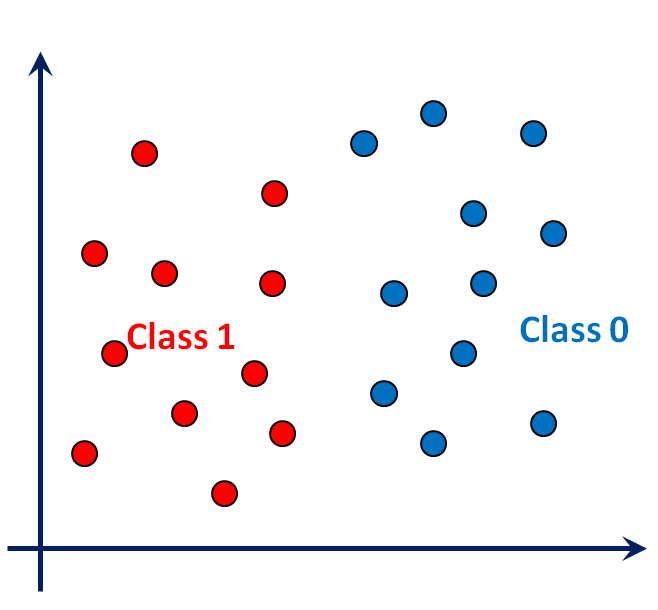
\includegraphics[width=0.8\textwidth]{Images/AIML_SVM_Linear_IMG1.png}}
		\only<2>{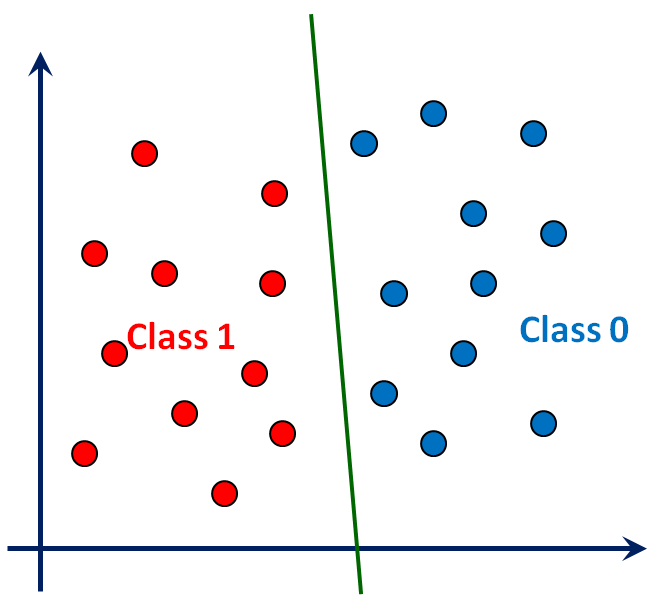
\includegraphics[width=0.8\textwidth]{Images/AIML_SVM_Linear_IMG2.png}}
		\only<3>{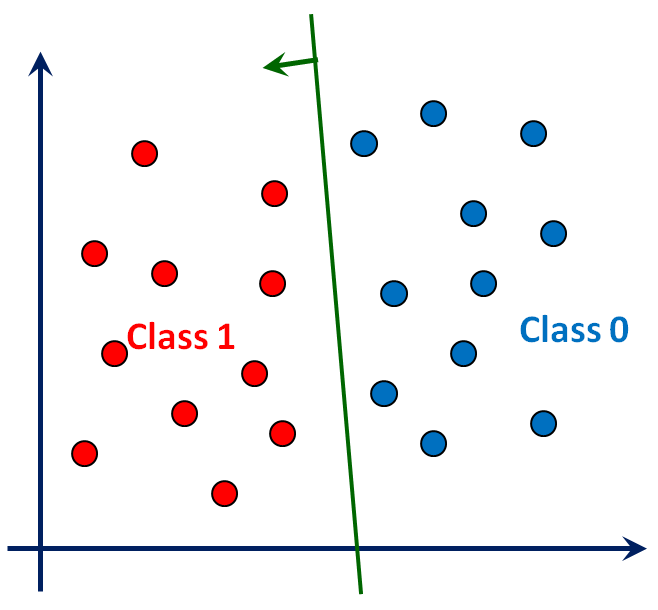
\includegraphics[width=0.8\textwidth]{Images/AIML_SVM_Linear_IMG3.png}}
		\end{overlayarea}
\end{column}
\end{columns}
\end{frame}


\begin{frame}{Why Linear? Generalization vs. Complexity}
	\begin{columns}
	\begin{column}{0.6\textwidth}
		
		\begin{overlayarea}{0.98\textwidth}{0.7\textheight}
			 \begin{itemize}
					 \only<4->{\vspace{-0.0cm}}
			\item Is it good to use a complex curve to reduce training error?\vspace{3cm}
		\end{itemize}
		\only<4->{\vspace{-2.4cm}\hspace{2cm}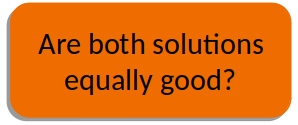
\includegraphics[width=0.5\textwidth]{Images/AIML_SVM_Linear_IMG9.png}}
			\vskip2cm
		\end{overlayarea}
		\end{column}
		\begin{column}{0.4\textwidth}
			\vspace{1cm}
			\begin{overlayarea}{0.98\textwidth}{0.65\textheight}
			\only<1>{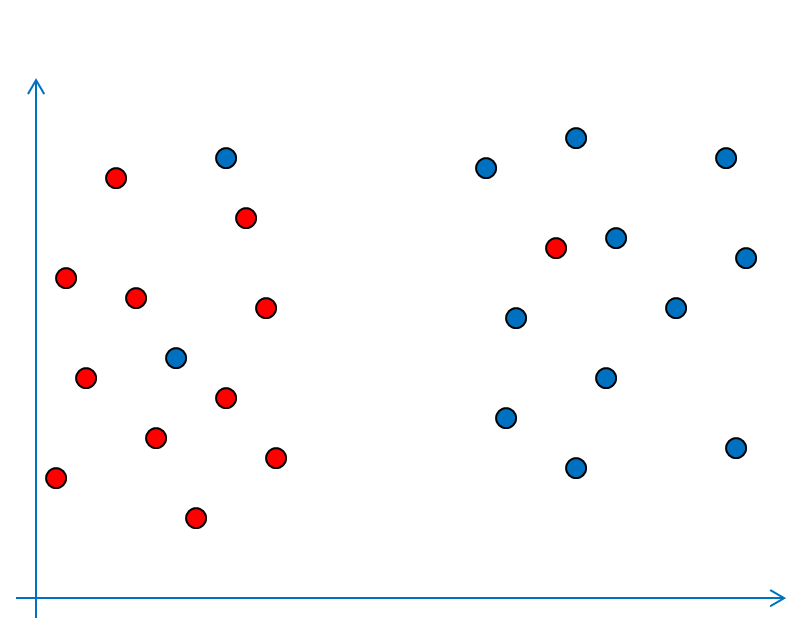
\includegraphics[width=0.98\textwidth]{Images/AIML_SVM_Linear_IMG4.png}}
			\only<2>{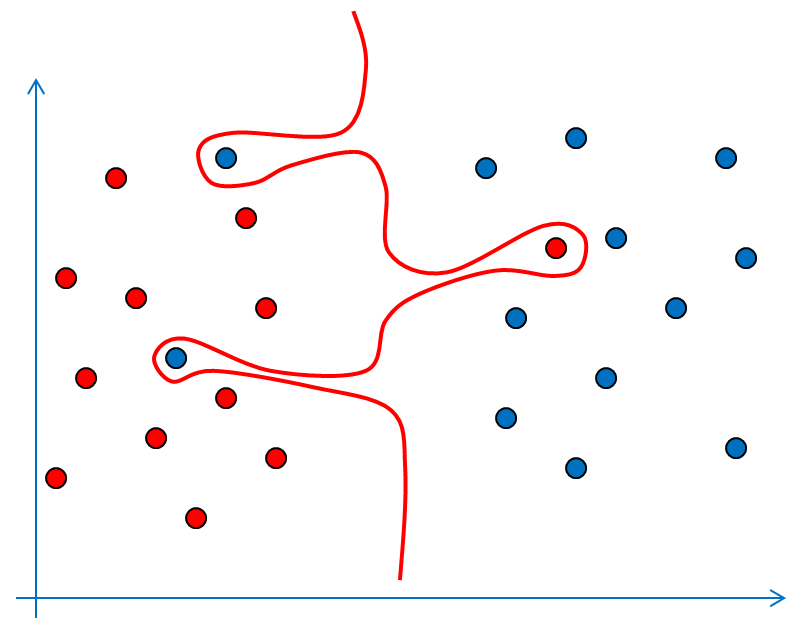
\includegraphics[width=0.98\textwidth]{Images/AIML_SVM_Linear_IMG5.png}}
			\only<3>{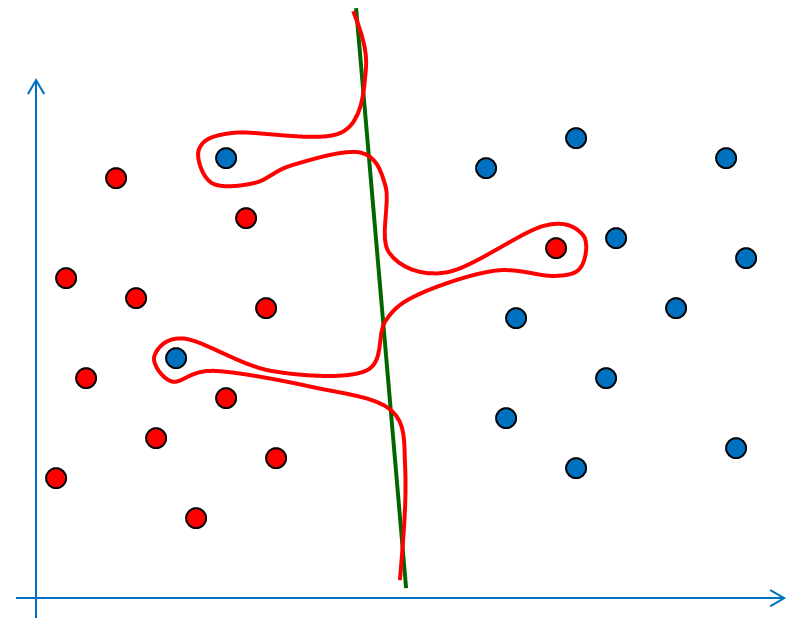
\includegraphics[width=0.98\textwidth]{Images/AIML_SVM_Linear_IMG6.png}}
			\only<4>{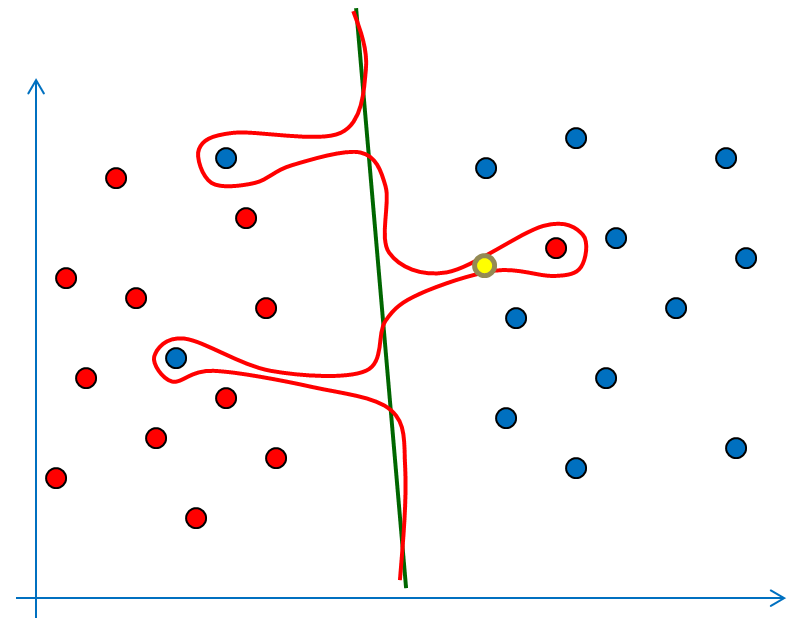
\includegraphics[width=0.98\textwidth]{Images/AIML_SVM_Linear_IMG7.png}}
			\only<5>{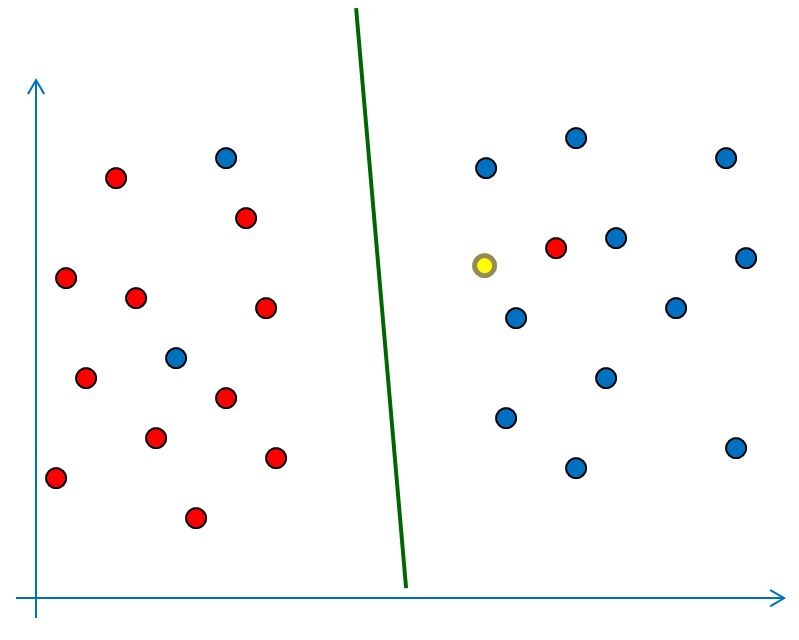
\includegraphics[width=0.98\textwidth]{Images/AIML_SVM_Linear_IMG8.png}}
			\only<6>{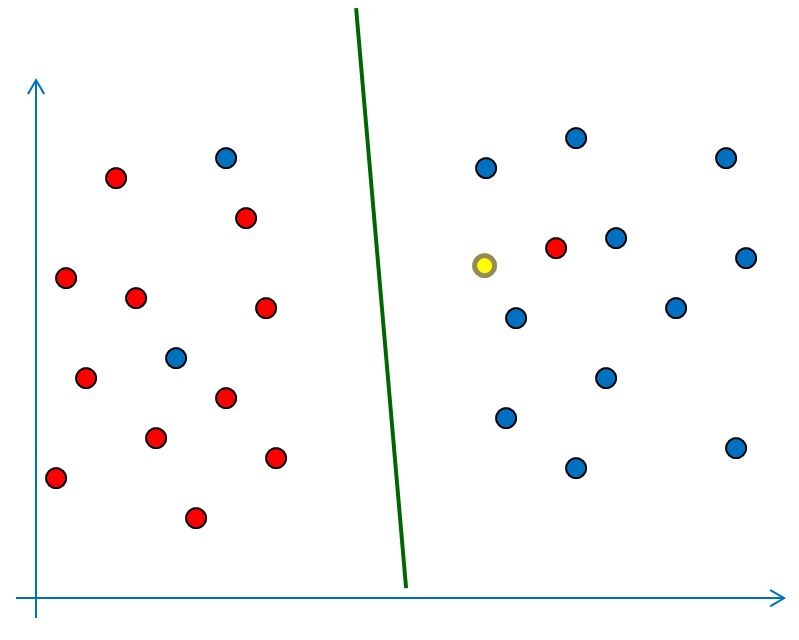
\includegraphics[width=0.98\textwidth]{Images/AIML_SVM_Linear_IMG8.png}} 
				\end{overlayarea}
			\end{column}
		\transwipe<2>[direction=270]
	\end{columns}
\end{frame}


\begin{frame}{Summary}
	\begin{itemize}
		\item Linear Classifiers are simple and hence efficient
		\item There exists simple learning algorithms
		\item Likely to work well for unseen test data (generalization)
		\item Can be converted to non-linear ones (later)
	\end{itemize}

\end{frame}



\begin{frame}{Perceptron Learning}
	\begin{columns}
		
		\begin{column}{0.6\textwidth}
		\vspace{-0.05cm}	\begin{itemize}
			\item<1-> Multiple solutions exist for linearly separable data
			\item<3-> Perceptron learning (any GD) results in a feasible solution \vspace{2cm}
			\end{itemize}
			\only<4->{\vspace{-2.2cm}\begin{center} 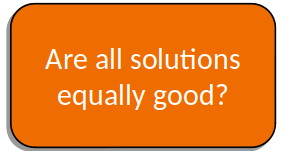
\includegraphics[width=4cm]{Images/AIML_SVM_Linear_IMG10.png} \end{center}} 
			\vspace{2cm}		
		\end{column}
		\begin{column}{0.4\textwidth}
			\begin{overlayarea}{\textwidth}{0.6\textheight}
			\only<1>{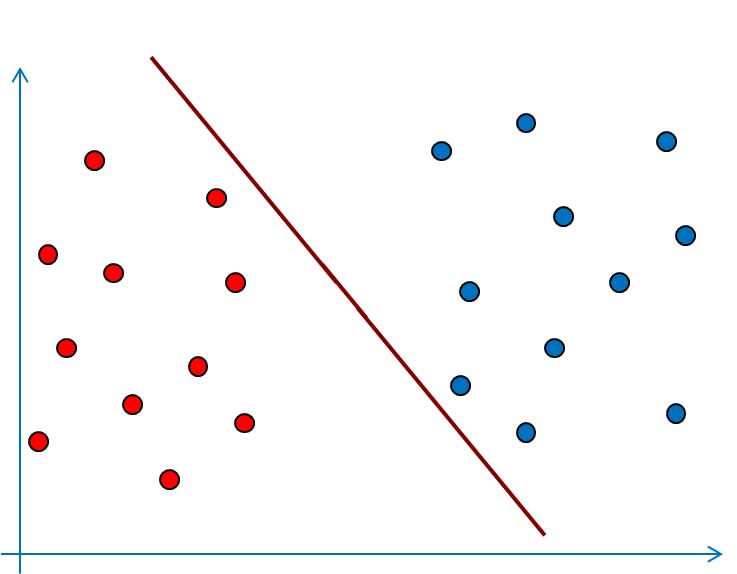
\includegraphics[width=\textwidth]{Images/AIML_SVM_Linear_IMG11.png}}
			\only<2>{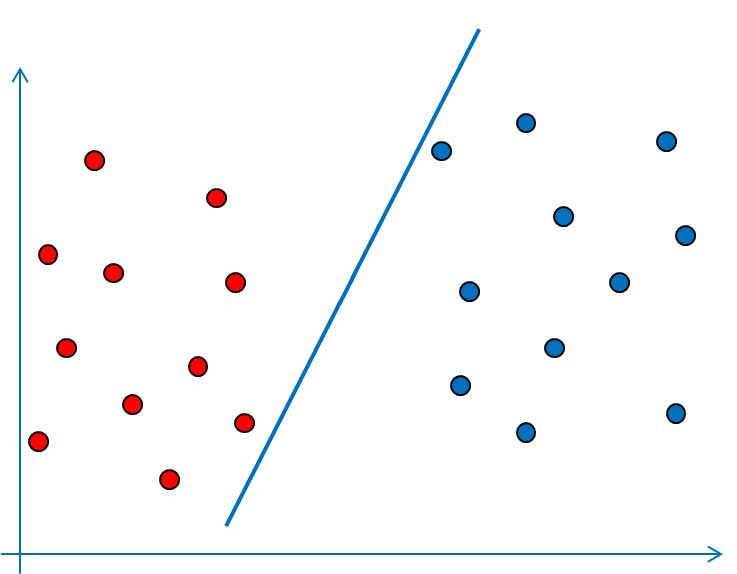
\includegraphics[width=\textwidth]{Images/AIML_SVM_Linear_IMG12.png}}
			\only<3>{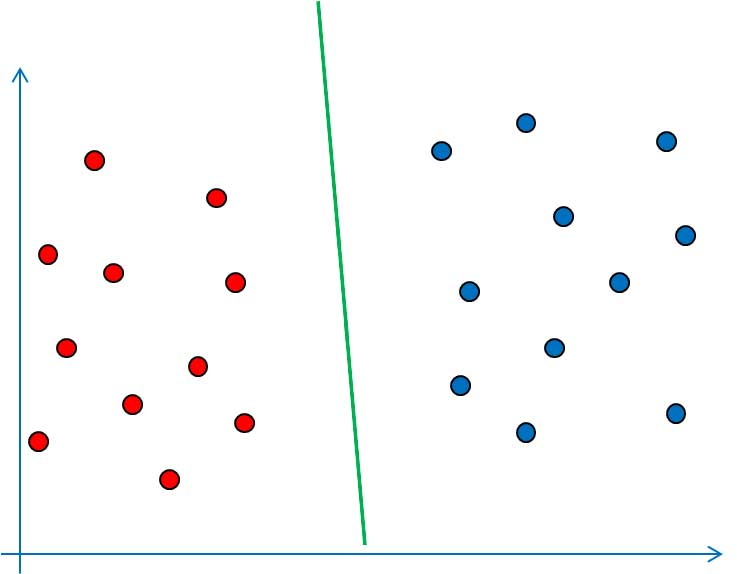
\includegraphics[width=\textwidth]{Images/AIML_SVM_Linear_IMG13.png}}
				\only<4>{\vspace{-0.97cm}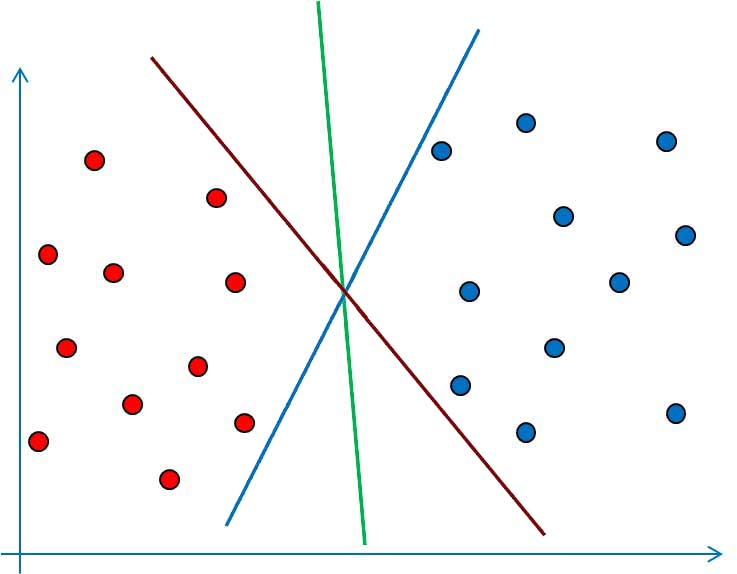
\includegraphics[width=\textwidth]{Images/AIML_SVM_Linear_IMG14.png}}
			\end{overlayarea}
\end{column}
	\end{columns}
\end{frame}



\begin{frame}{Margin: The No-mans Band}
	\begin{columns}
		\begin{column}{0.55\textwidth}
			\begin{itemize}
		\item<1-> \alert{Margin:} Width of a band around decision boundary without any training samples
		\item<3-> Margin varies with the position and orientation of the separating hyperplane
		\end{itemize}
			\only<4->{\begin{center} 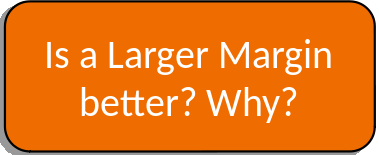
\includegraphics[width=4cm, height=1.3cm]{Images/AIML_SVM_Linear_IMG15.png}\vspace{1cm}\end{center}}
%			\only<4->{\vspace{-0.4cm}\begin{center} \begin{tcolorbox}[width=3.5cm,left=0pt, right=0pt,colframe=black,height=1.5cm, colback=orange]
%                               \textcolor{white}{\small{Is a Larger Margin better? Why?}}
%		\end{tcolorbox} \end{center} }
			\vspace{2cm}
		\end{column}
		\begin{column}{0.45\textwidth}
			\begin{overlayarea}{\textwidth}{0.65\textheight}
			\only<1>{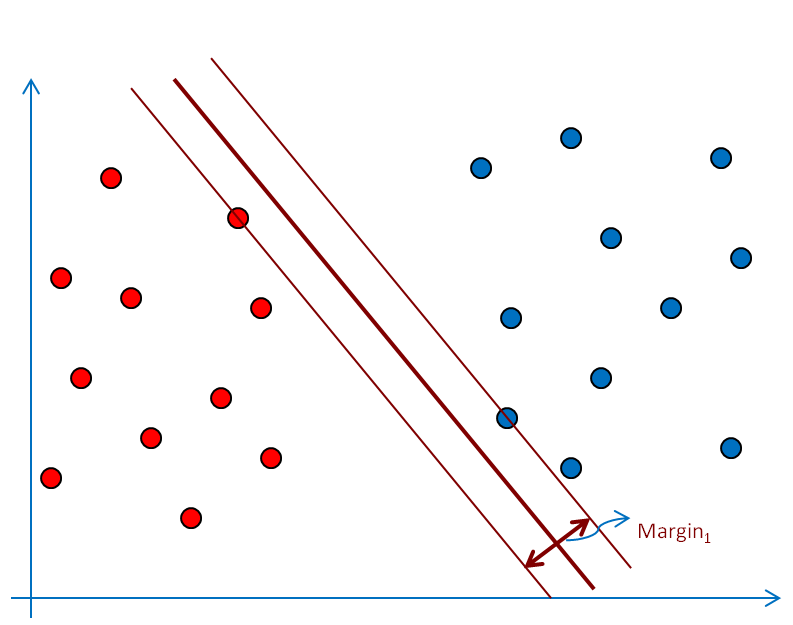
\includegraphics[width=0.9\textwidth]{Images/AIML_SVM_Linear_IMG16.png}}
			\only<2>{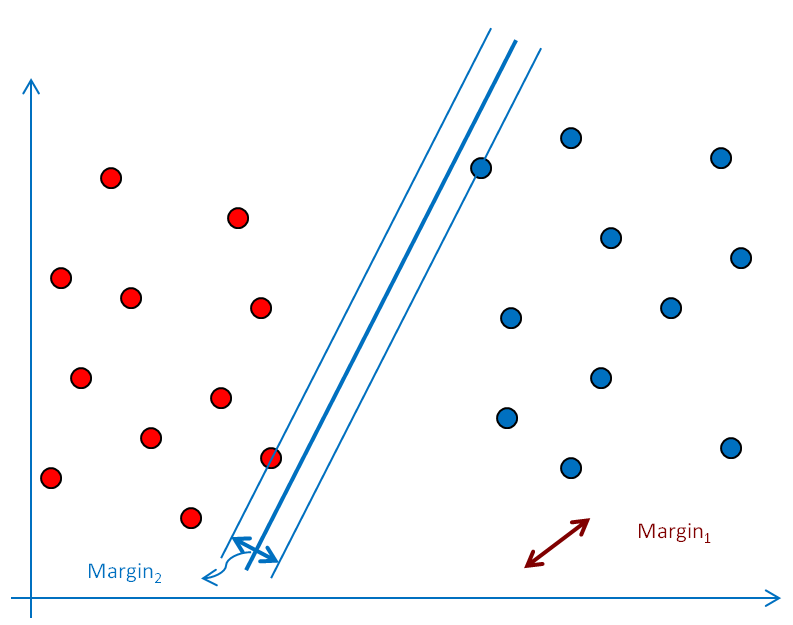
\includegraphics[width=0.9\textwidth]{Images/AIML_SVM_Linear_IMG17.png}}
			\only<3>{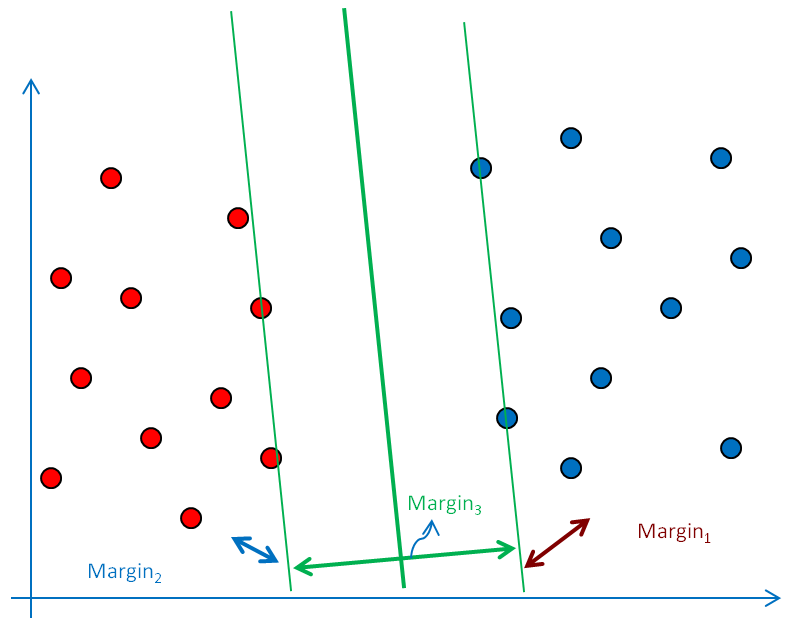
\includegraphics[width=0.9\textwidth]{Images/AIML_SVM_Linear_IMG18.png}}
				\only<4>{\vspace{-2.05cm}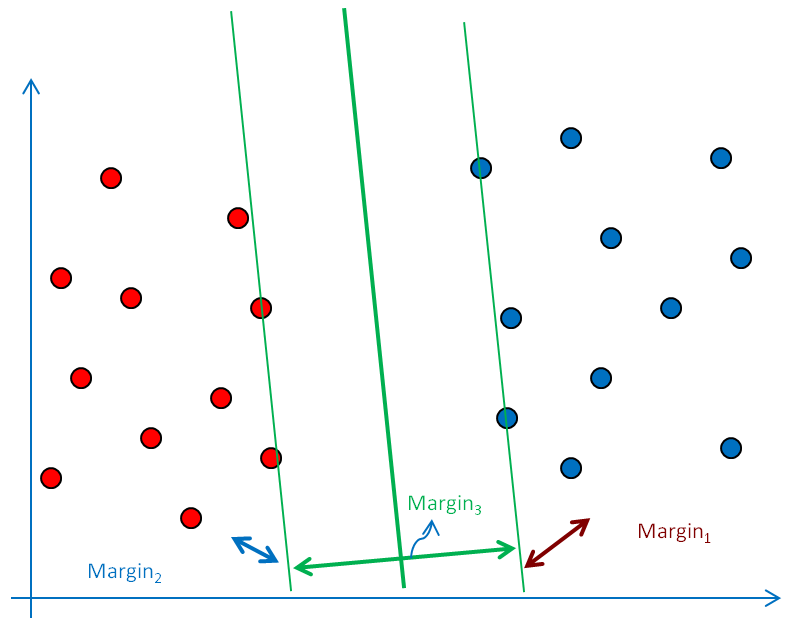
\includegraphics[width=0.9\textwidth]{Images/AIML_SVM_Linear_IMG18.png}}
			\end{overlayarea}
		\end{column}
	\end{columns}

\end{frame}

\begin{frame}{Why Maximize Margin?}
        \begin{columns}
                \begin{column}{0.5\textwidth}
		\begin{overlayarea}{\textwidth}{0.65\textheight}
			\begin{itemize}
			\item Test samples vary from training data
			\item What is their chance of being misclassified?
     			\end{itemize}
			\only<6->{\hspace{1.5cm}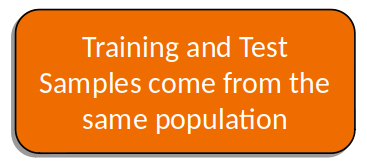
\includegraphics[width=0.5\textwidth]{Images/AIML_SVM_Linear_IMG24.png}}
%		\vspace{2cm}
		\end{overlayarea}
		\end{column}
		\begin{column}{0.5\textwidth}
			\begin{overlayarea}{\textwidth}{0.65\textheight}
			\only<1>{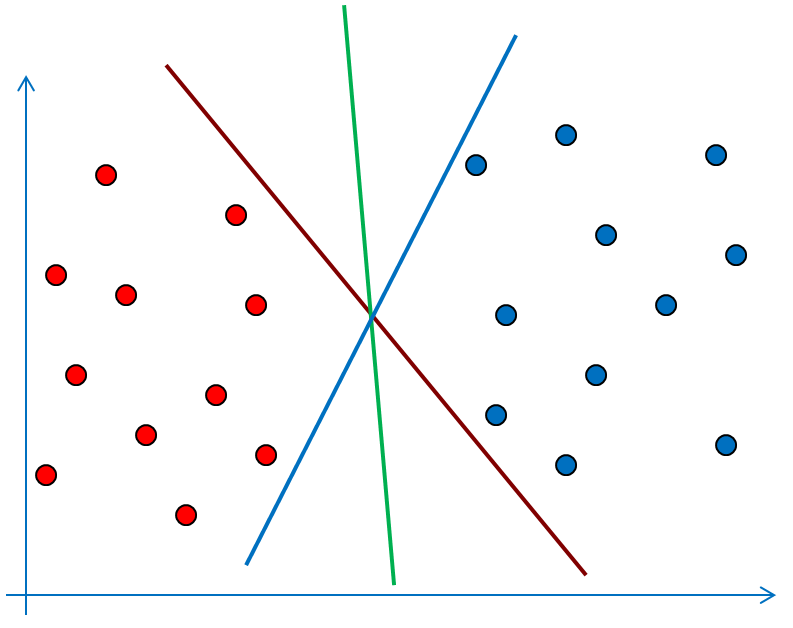
\includegraphics[width=\textwidth]{Images/AIML_SVM_Linear_IMG19.png}}
			\only<2>{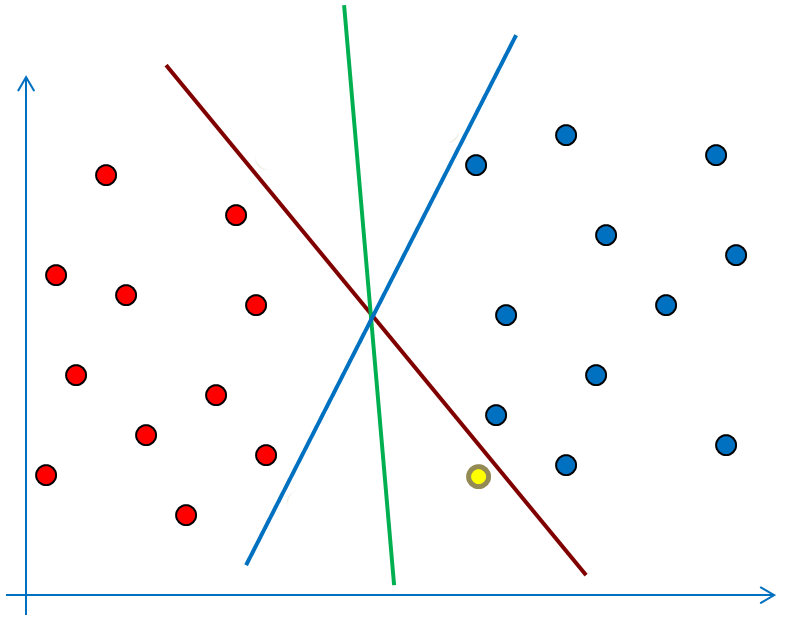
\includegraphics[width=\textwidth]{Images/AIML_SVM_Linear_IMG20.png}}
			\only<3>{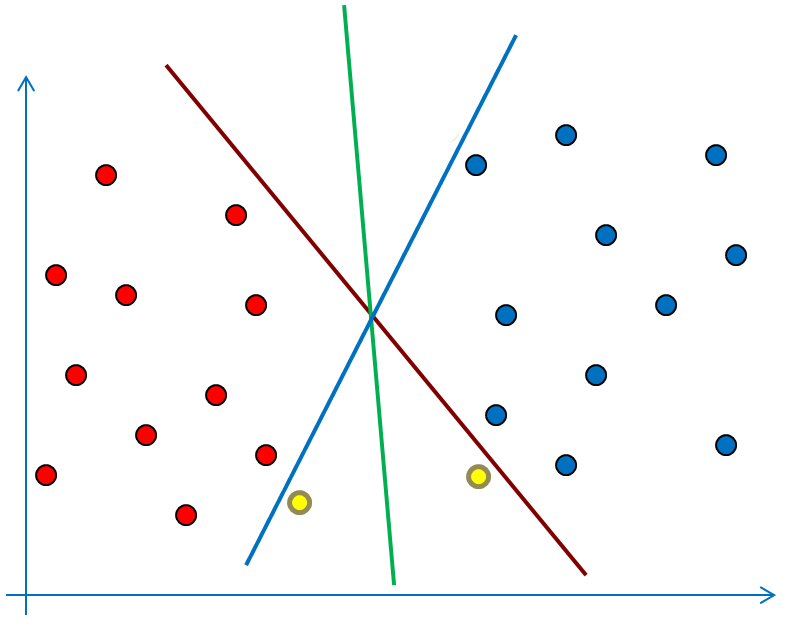
\includegraphics[width=\textwidth]{Images/AIML_SVM_Linear_IMG21.png}}
			\only<4>{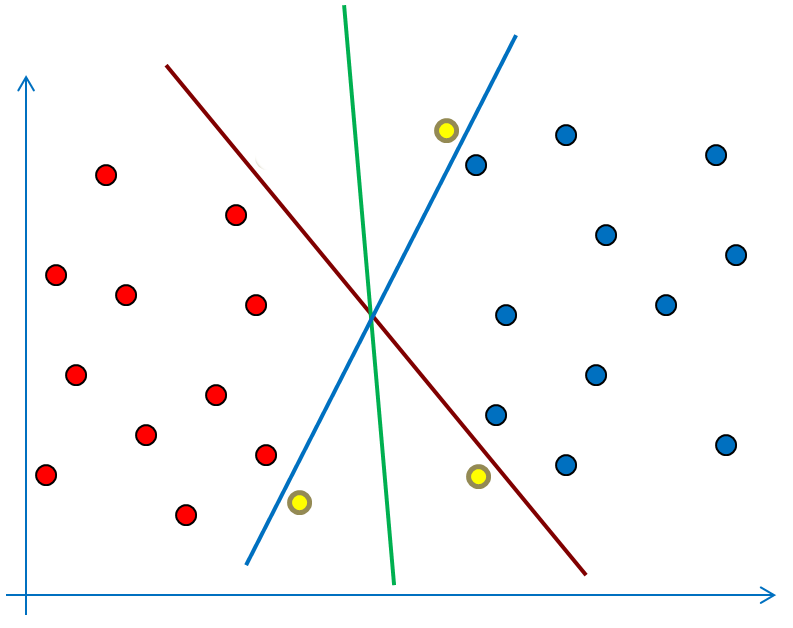
\includegraphics[width=\textwidth]{Images/AIML_SVM_Linear_IMG22.png}}
			\only<5->{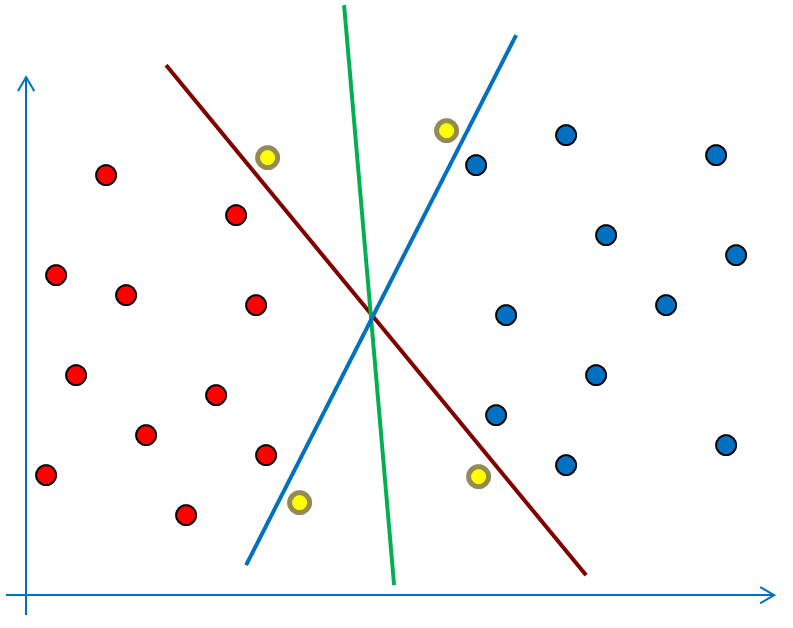
\includegraphics[width=\textwidth]{Images/AIML_SVM_Linear_IMG23.png}}
			\transduration<2-4>{0.2}
			\end{overlayarea}
		\end{column}

\end{columns}
\end{frame}




\begin{frame}{Summary: Max-Margin Classification}
	\begin{columns}
		\begin{column}{0.55\textwidth}
	\begin{itemize}
		\item A Large Margin will reduce the chance of misclassifying future test samples
		\item In other words, large-margin classifiers will generalize better.
	\end{itemize}
		\end{column}
		\begin{column}{0.45\textwidth}
			\begin{overlayarea}{\textwidth}{0.65\textheight}
				\only<1>{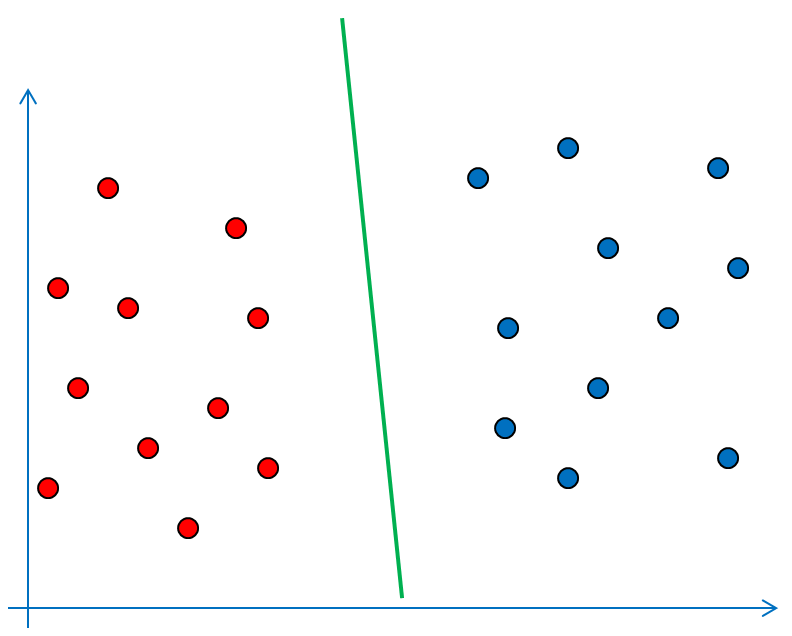
\includegraphics[width=\textwidth]{Images/AIML_SVM_Linear_IMG25.png}}
				\only<2>{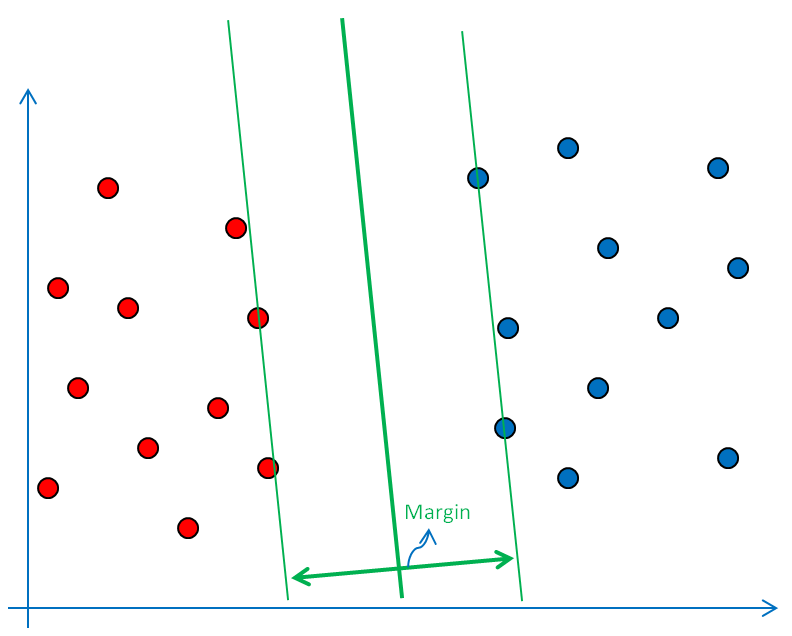
\includegraphics[width=\textwidth]{Images/AIML_SVM_Linear_IMG26.png}}
			
				\only<3>{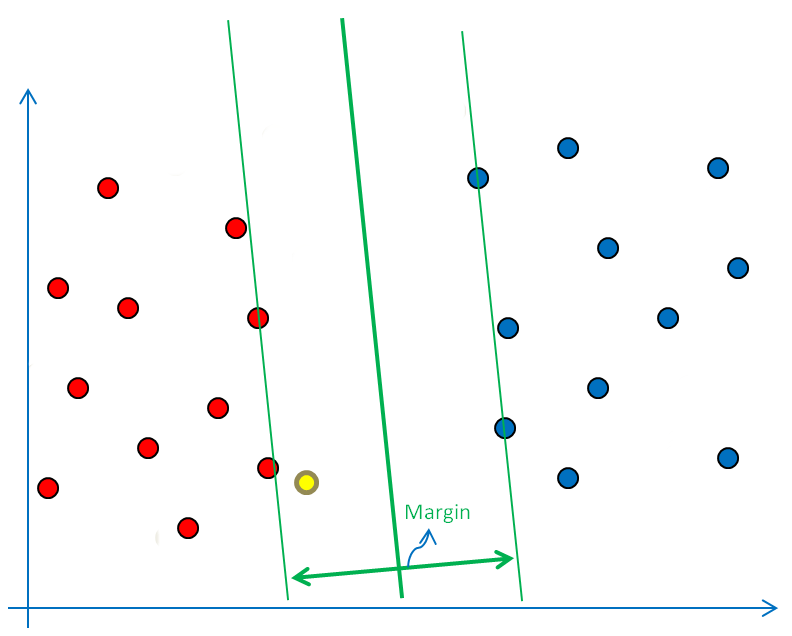
\includegraphics[width=\textwidth]{Images/AIML_SVM_Linear_IMG29.png}}
			\only<4>{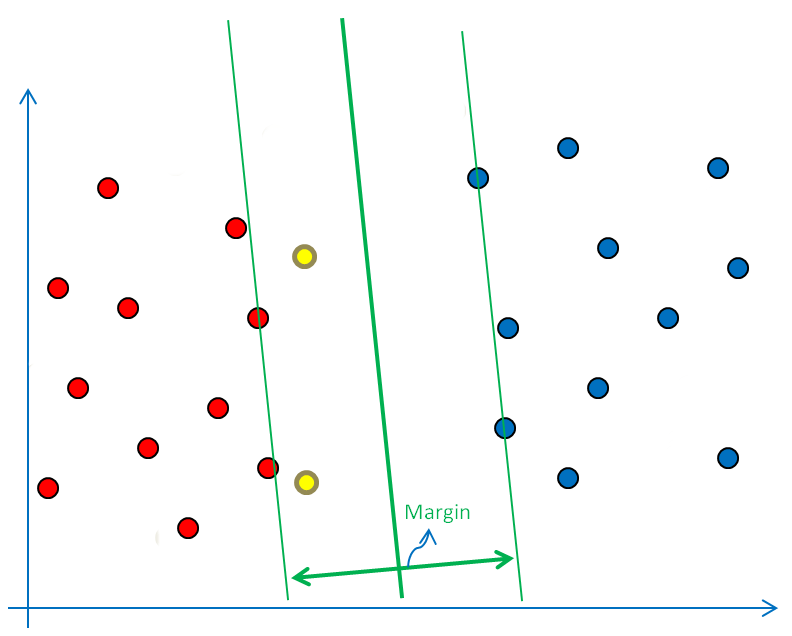
\includegraphics[width=\textwidth]{Images/AIML_SVM_Linear_IMG30.png}}
			\only<5>{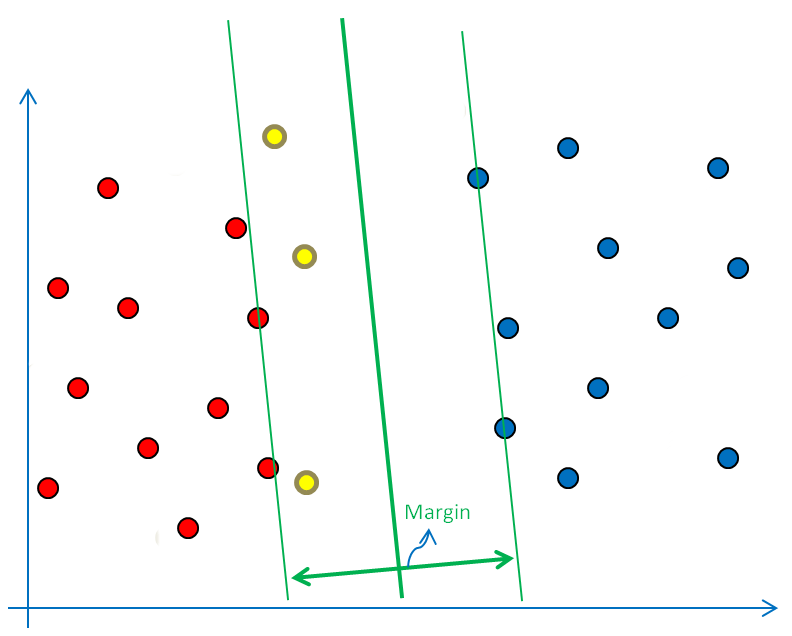
\includegraphics[width=\textwidth]{Images/AIML_SVM_Linear_IMG31.png}}
			\only<6>{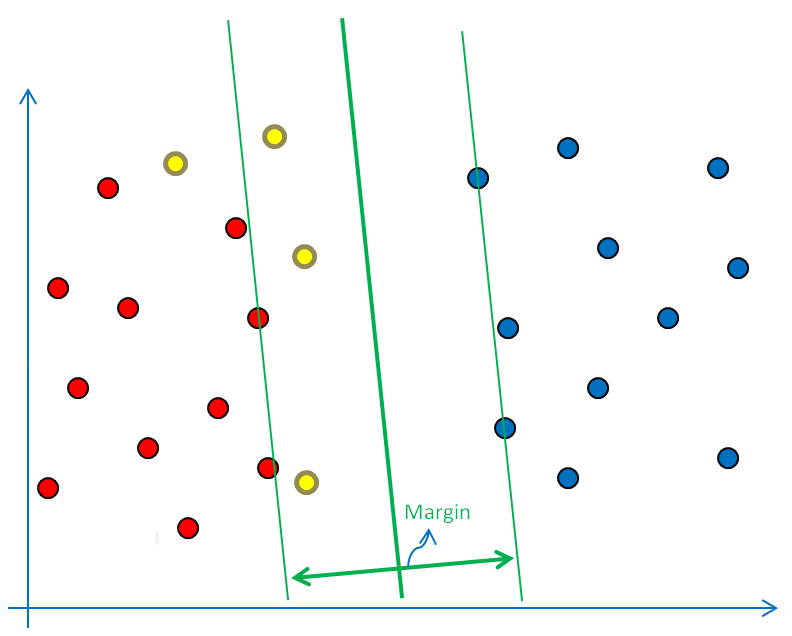
\includegraphics[width=\textwidth]{Images/AIML_SVM_Linear_IMG32.png}}
			\only<7>{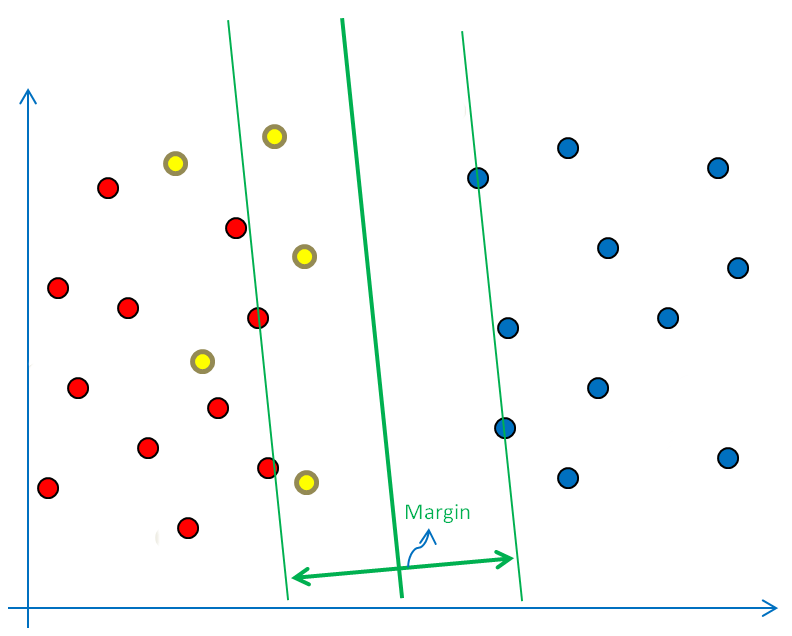
\includegraphics[width=\textwidth]{Images/AIML_SVM_Linear_IMG33.png}}
			\only<8>{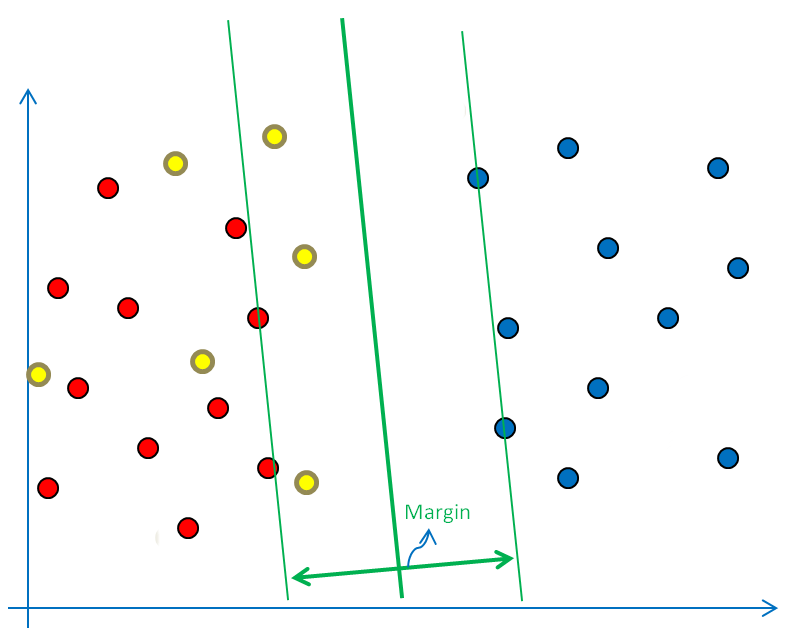
\includegraphics[width=\textwidth]{Images/AIML_SVM_Linear_IMG34.png}}
			\only<9>{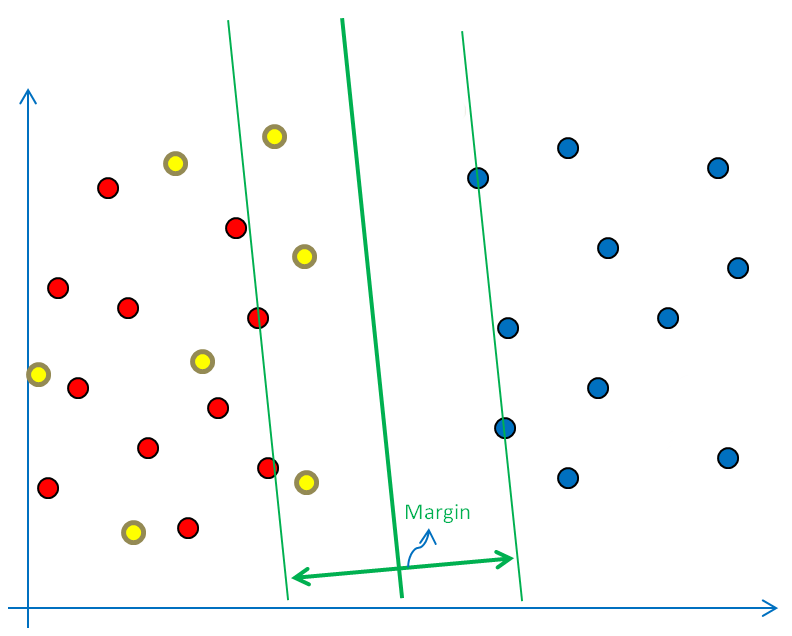
\includegraphics[width=\textwidth]{Images/AIML_SVM_Linear_IMG35.png}}
			\only<10>{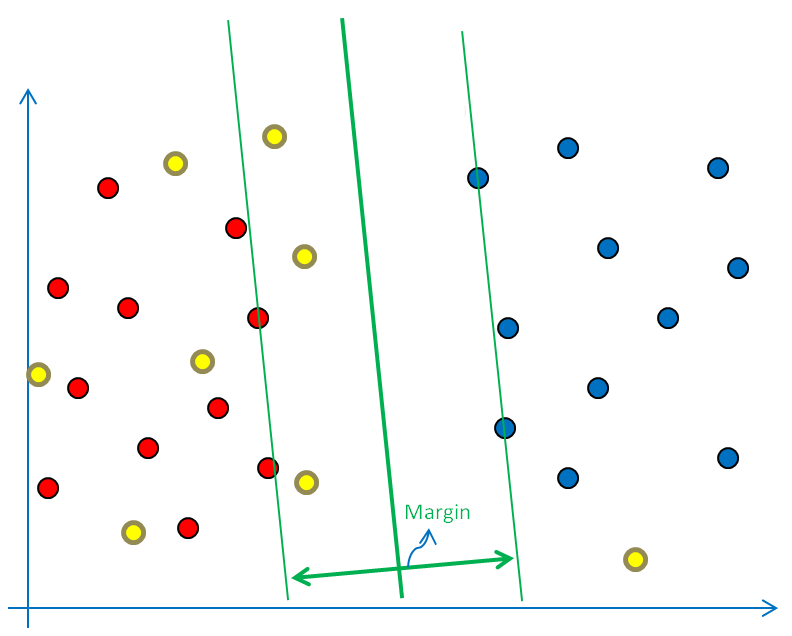
\includegraphics[width=\textwidth]{Images/AIML_SVM_Linear_IMG36.png}}
			\only<11>{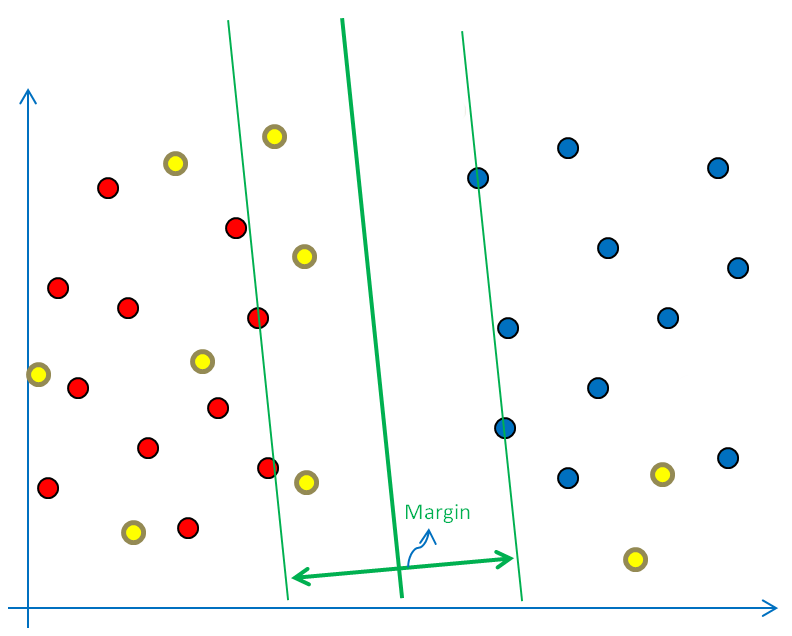
\includegraphics[width=\textwidth]{Images/AIML_SVM_Linear_IMG37.png}}
			\only<12>{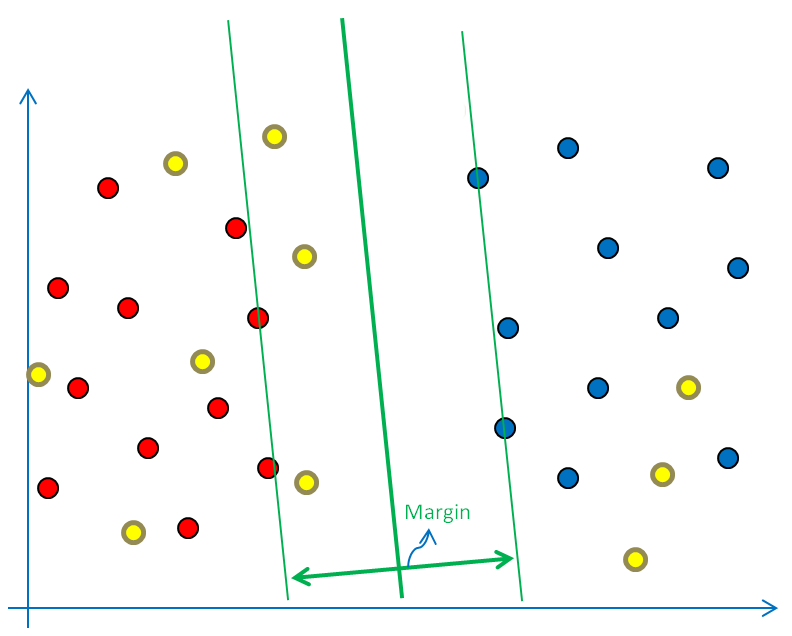
\includegraphics[width=\textwidth]{Images/AIML_SVM_Linear_IMG38.png}}
			\only<13>{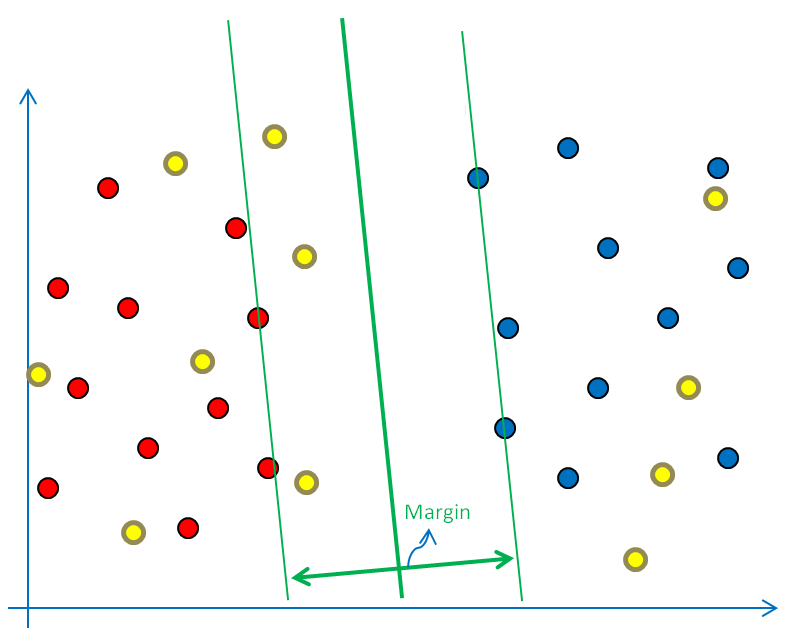
\includegraphics[width=\textwidth]{Images/AIML_SVM_Linear_IMG39.png}}
			\only<14>{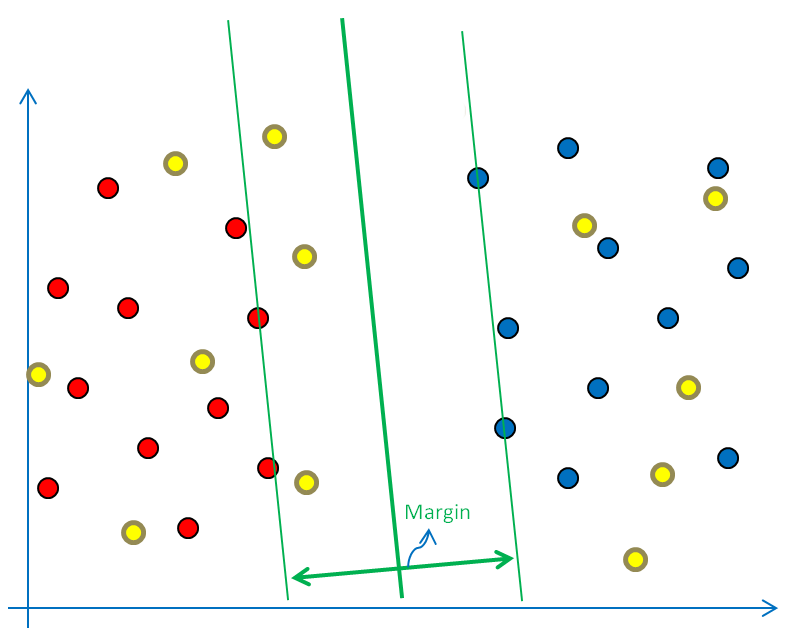
\includegraphics[width=\textwidth]{Images/AIML_SVM_Linear_IMG40.png}}
			\only<15>{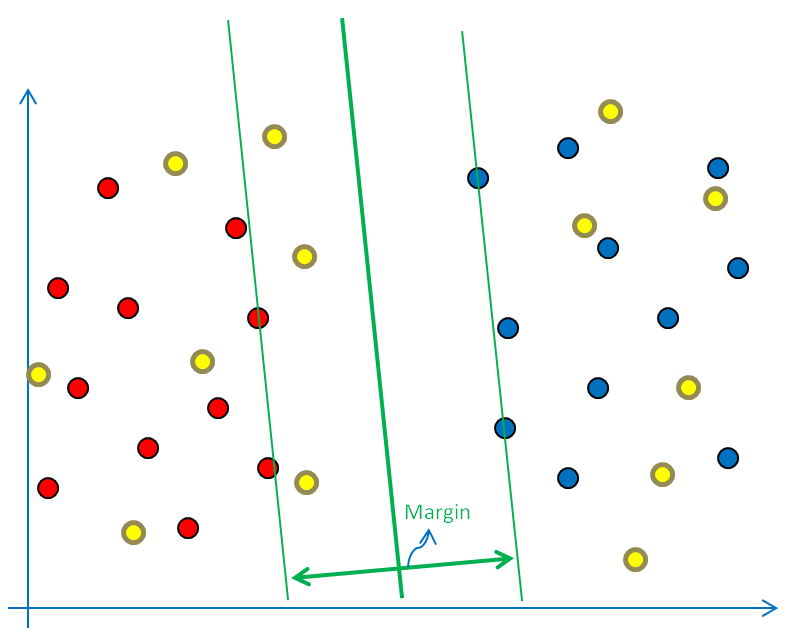
\includegraphics[width=\textwidth]{Images/AIML_SVM_Linear_IMG41.png}}
			\only<16>{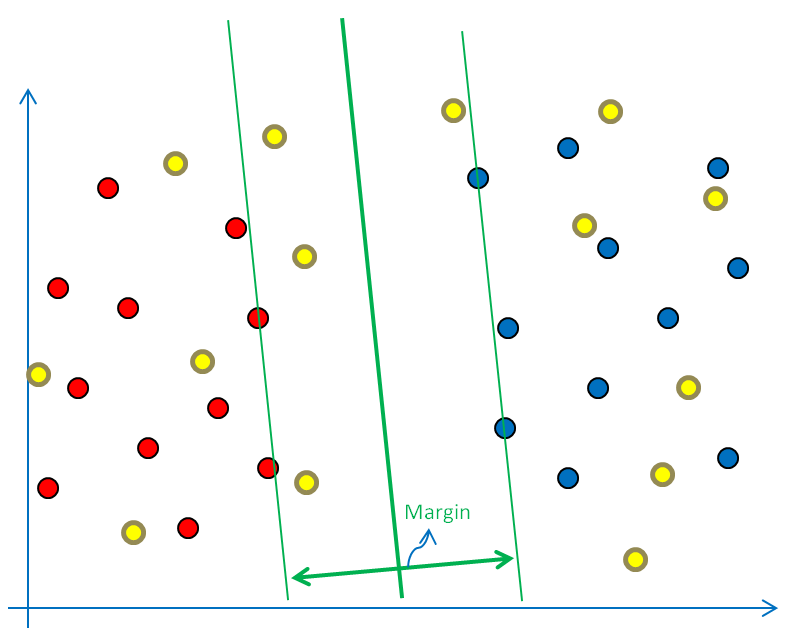
\includegraphics[width=\textwidth]{Images/AIML_SVM_Linear_IMG42.png}}
			 \only<17>{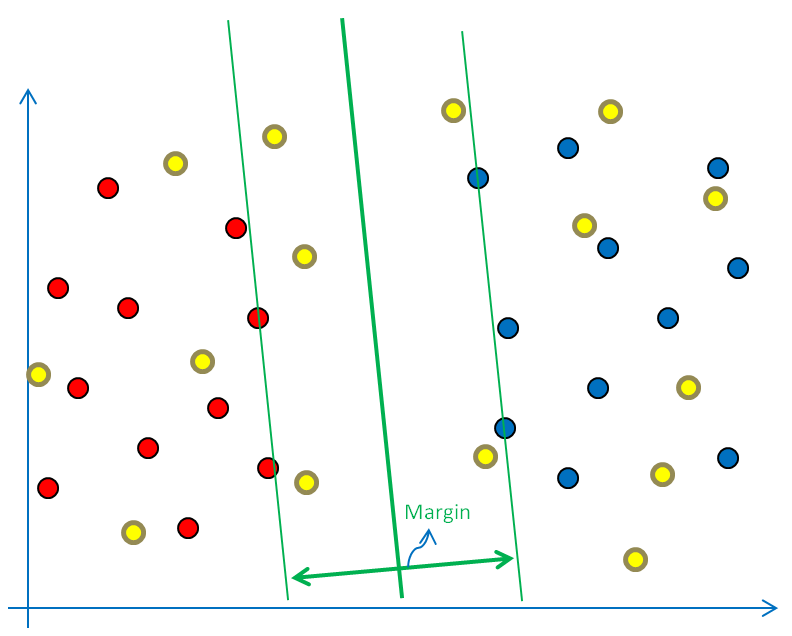
\includegraphics[width=\textwidth]{Images/AIML_SVM_Linear_IMG43.png}}
			\only<18>{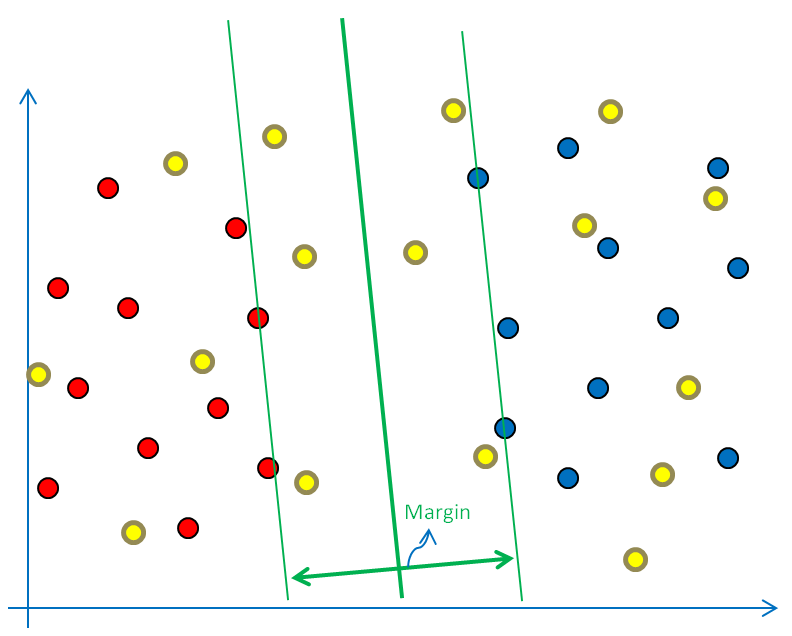
\includegraphics[width=\textwidth]{Images/AIML_SVM_Linear_IMG44.png}}
			\transduration<3-17>{-0.0}
			\end{overlayarea}
		\end{column}
	\end{columns}
\end{frame}


\begin{frame}{Summary: Max-Margin Classification}
	\begin{columns}
		\begin{column}{0.55\textwidth}
	\begin{itemize}
		\item A Large Margin will reduce the chance of misclassifying future test samples
		\item In other words, large-margin classifiers will generalize better
                \item Samples at the boundary support the margin: called Support Vectors
	\end{itemize}
		\end{column}
		\begin{column}{0.45\textwidth}
			\begin{overlayarea}{\textwidth}{0.65\textheight}
				\only<1>{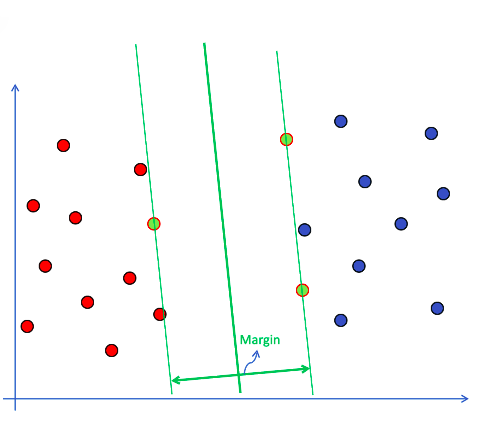
\includegraphics[width=\textwidth]{Images/AIML_SVM_Linear_IMG27.png}}
				\only<2>{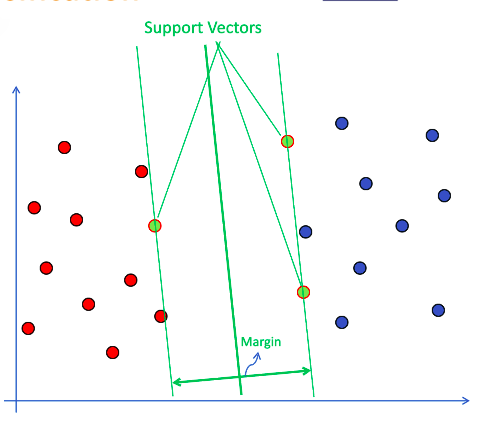
\includegraphics[width=\textwidth]{Images/AIML_SVM_Linear_IMG28.png}}
			
			\end{overlayarea}
		\end{column}
	\end{columns}
\end{frame}





\begin{frame}{Summary}
		\begin{itemize}
			\item SVMs are very good at generalization
			\item Convex optimization. No worries about local minima.
			\item Many excellent solvers. (Often we never code ourselves.)
			\item Linear SVMs are efficient for training and testing (both memory and flops).
			\item They are also highly accurate
		\end{itemize}
\end{frame}


\end{document}
